\begin{figure}
	\centering
	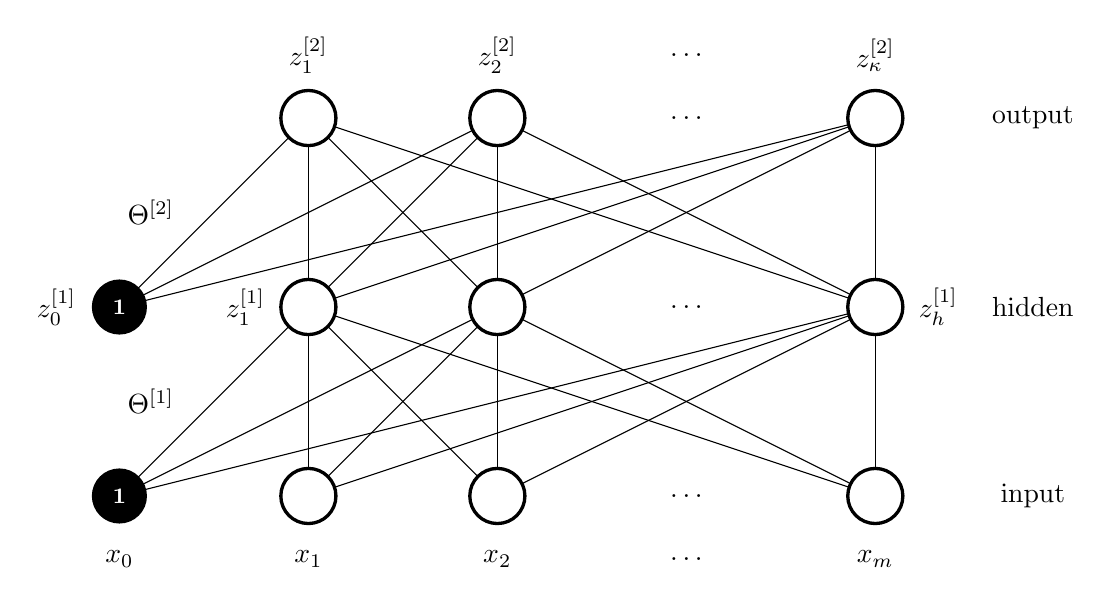
\begin{tikzpicture}[
		scale=0.8,
		b/.style={circle,fill=black,minimum width=7mm},
		n/.style={circle,draw=black,fill=white,very thick,minimum width=7mm}
	]
		
		\foreach \y in {3,6}{
			\foreach \i in {-4.5,-1.5,1.5,7.5}{
				\foreach \j in {-1.5,1.5,7.5}{
					\draw (\i, \y-3) -- (\j,\y);
				}
			}
		}
		
		% input layer
		\node[b] at (-4.5,0) {\footnotesize\textcolor{white}{\textbf{1}}};
		\node[n] at (-1.5,0) {};
		\node[n] at (1.5,0) {};
		\node at (4.5,0) {$\dots$};
		\node[n] at (7.5,0) {};

		% hidden layer
		\node[b] at (-4.5,3) {\footnotesize\textcolor{white}{\textbf{1}}};
		\node[n] at (-1.5,3) {};
		\node[n] at (1.5,3) {};
		\node at (4.5,3) {$\dots$};
		\node[n] at (7.5,3) {};

		% output layer
		\node[n] at (-1.5,6) {};
		\node[n] at (1.5,6) {};
		\node at (4.5,6) {$\dots$};
		\node[n] at (7.5,6) {};

		% input
		\node at (-4.5,-1) {$x_0$};
		\node at (-1.5,-1) {$x_1$};
		\node at (1.5,-1) {$x_2$};
		\node at (4.5,-1) {$\dots$};
		\node at (7.5,-1) {$x_m$};
		
		% output
		\node at (-1.5,7) {$z_1^{[2]}$};
		\node at (1.5,7) {$z_2^{[2]}$};
		\node at (4.5,7) {$\dots$};
		\node at (7.5,7) {$z_\kappa^{[2]}$};

		% hidden
		\node at (-5.5,3) {$z_0^{[1]}$};
		\node at (-2.5,3) {$z_1^{[1]}$};
		\node at (8.5,3) {$z_h^{[1]}$};

		% weights
		\node at (-4,1.5) {$\bm{\Theta}^{[1]}$};
		\node at (-4,4.5) {$\bm{\Theta}^{[2]}$};
		
		\node at (10,0) {\highlight{input}};
		\node at (10,3) {\highlight{hidden}};
		\node at (10,6) {\highlight{output}};
		
	\end{tikzpicture}
\end{figure}